\documentclass[12pt,letterpaper]{article}
\usepackage[margin=1.5in]{geometry}
\usepackage[english]{babel}
\usepackage[utf8x]{inputenc}
\usepackage{amsmath}
\usepackage{amssymb} 
\usepackage[retainorgcmds]{IEEEtrantools}
\usepackage{graphicx}
\usepackage{tabularx}
\usepackage{subfig}
\usepackage{kpfonts}    % for nice fonts
\usepackage{microtype} 
\usepackage{booktabs}   % for nice tables
\usepackage{bm}         % for bold math
\usepackage{listings}   % for inserting code
\usepackage{verbatim}   % useful for program listings
\usepackage{color}  
\usepackage[colorlinks=true]{hyperref}
% use for hypertext
\usepackage[colorinlistoftodos]{todonotes}
\usepackage{natbib}

\hypersetup{
    colorlinks=true,
    linkcolor=blue, 
    filecolor=magenta, 
    urlcolor=cyan,
    citecolor=magenta 
}

\begin{document}

\section{Short Summary}

The main contents of this report are the same as the last version. Below are some key differences and results:

\begin{itemize}
    \item One mistake in the last report is that I misspecify the structure of Nash Equilibriums. In the last report, I missed multiple pure-strategy NEs situations and concluded that there is no mixed-strategy NE. In fact, most tabular game has only one unique pure-strategy NE, in which case the computation under Equations \ref{eq:solutions} can give results beyond $[0,1]$. In this new report, the decision-making process for both firms is given below (public capacity setting):
    \begin{enumerate}
        \item Find whether there exists a \textbf{unique} pure-strategy NE, if exists, then pick it as the action pair;
        \item If not exists (multiple pure-strategy NEs or no pure-strategy NE), solving the mixed-strategy solution using equations \ref{eq:solutions}.
    \end{enumerate}
    The average difference of $V_i$ at each state under the two different approaches is $0.032$.

    \item Following the framework in the previous report, new dynamic programming $W_i(s_i,s_{-i},\cdot,\cdot,t)$ can be used to calculate the expected payoff for a single firm under pre-assumed decision-making process. When both firms have the same initial capacity, the numerical results are similar to that of the last report, i.e., the value function is usually higher in the transparent-capacity setting\footnote{In fact, the gap of value function between the opaque and transparent-capacity setting is larger in this renewed version, this is due to that I misclassified some mixed-strategy NE as pure-strategy NE, and my code logic is to select $(p_h,p_h)$ as the equilibrium when there are multiple pure-strategy NE, which could bring more revenue for both firms.}. (see detailed graphs given in Subsection \ref{subsec:symmetric}).

    When both firms over-estimate the opponent's initial capacity, the payoffs between the transparent and opaque settings have the smallest difference.

    \item Comparisons under asymmetric initial capacities, figure \ref{fig:ratio6} depicts the case when firm $i$ has higher initial capacity and figure \ref{fig:ratio7} depicts the case when firm $i$ has lower initial capacity. The results show that the transparent-capacity setting is beneficial for both firms in asymmetric cases.
\end{itemize}

\begin{figure}
    \centering
    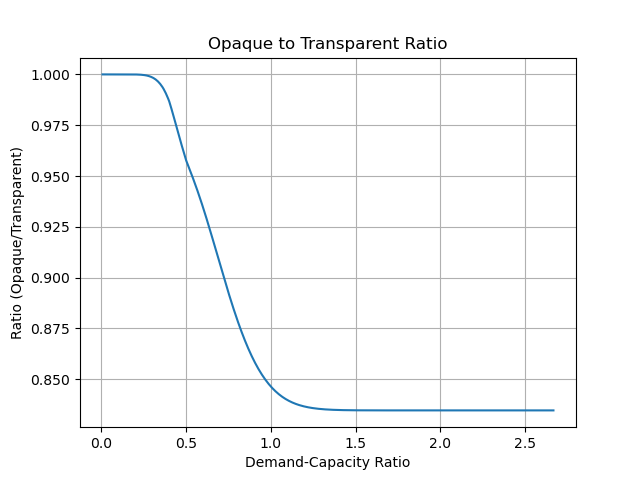
\includegraphics[width=0.5\linewidth]{pic/0930_ratio6.png}
    \caption{$W_i(10,20,10,20,t)$ v.s. $V_i(10,20,t)$}
    \label{fig:ratio6}
\end{figure}

\begin{figure}
    \centering
    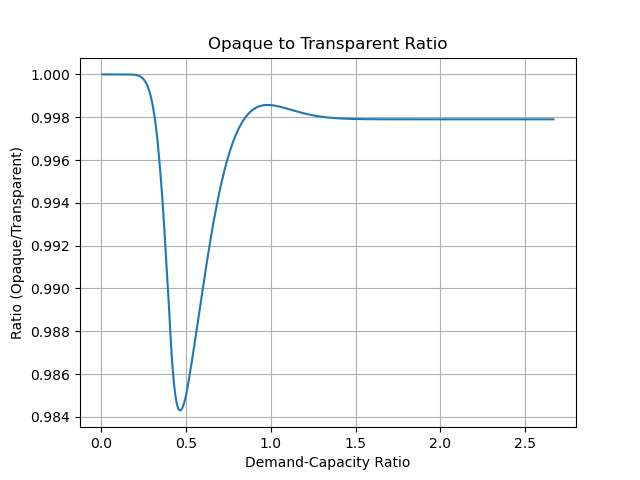
\includegraphics[width=0.5\linewidth]{pic/0930_ratio7.png}
    \caption{$W_i(20,10,20,10,t)$ v.s. $V_i(20,10,t)$}
    \label{fig:ratio7}
\end{figure}

\section{Model \& Assumptions}

We assume there are two \textit{symmetric} firms indexed by $i\in\{1,-1\}$ competing on prices given a finite discrete horizon $t=\{T,T-1,\cdots,1,0\}$. At each time $t$, each firm $i$ can set price $p_{it}\in\{p_l,p_h\}$\footnote{This simplification borrows from \cite{miklos2019collusion}.}, where $0<p_l<p_h$. The price vector is denoted by $p_t$. 

Each period, there is a potential customer with probability $\lambda<1$, and we assume the demand follows the logit function:

\[
    q_i(p_t) = \frac{\exp(a-bp_i)}{1+\sum_{i\in\{1,-1\}}\exp(a-bp_i) }
\]

where $a, b$ should satisfy $a>0, b>0$.

For simplicity, we could write the purchasing probability as:

\[
    q_{ll} = \frac{\exp(a-bp_l)}{1+2\exp(a-bp_l)}, q_{lh} = \frac{\exp(a-bp_l)}{1+\exp(a-bp_l)+\exp(a-bp_h)};
\]

\[
    q_{hl} = \frac{\exp(a-bp_h)}{1+\exp(a-bp_l)+\exp(a-bp_h)}, q_{hh} = \frac{\exp(a-bp_h)}{1+2\exp(a-bp_h)}.
\]

i.e. $q_{xy}$ denotes the demand function for firm $i$ when the price vector $(p_i,p_{-i})$ is $p_x,p_y$. 

At time $T$, each firm has a public initial capacity $s\ge0$. 

\section{Capacity as Public Information}

Denote $V_i(s_i, s_{-i}, t)$ as the value function given the current state $(s_i, s_{-i}, t)$ when both firms adopt the equilibrium prices. When one customer arrives at time $t$ and firm $i,-i$ set their prices at $p_x, p_y$ respectively, the revenue pair $\pi(p_x,p_y, ,s_i,s_{-i},t) = (\pi_i(p_x,p_y,s_i,s_{-i},t), \pi_{-i}(p_x,p_y,s_i,s_{-i},t))$ is given by:

\begin{align}
    \pi_i(p_x,p_y,s_i,s_{-i},t) &= q_{xy}\cdot (p_x+V_i(s_i-1,s_{-i},t-1)) + q_{yx}\cdot V_i(s_i, s_{-i}-1, t-1) \nonumber \\
    &\quad + (1-q_{xy}-q_{yx}) \cdot V_i(s_i,s_{-i},t-1) \nonumber \\
    \pi_{-i}(p_x,p_y,s_i,s_{-i},t) &= q_{xy}\cdot V_i(s_{-i}, s_i-1, t-1) + q_{yx}\cdot (p_y+V_i(s_{-i}-1, s_i, t-1)) \nonumber \\
    &\quad + (1-q_{xy}-q_{yx}) \cdot V_i(s_{-i},s_{i},t-1) \label{eq:revenue_pair}
\end{align}
    
Under the equilibrium price $p_x^*(s_i,s_{-i},t),p_y^*(s_i,s_{-i},t)$, the value function can be expressed by:

\begin{equation}\label{eq:value_function}
    V_i(s_i,s_{-i},t) =& \lambda \pi_i(p_x^*,p_y^*,s_i,s_{-i},t) + (1-\lambda) V_i(s_i,s_{-i},t-1) 
\end{equation}

The boundary condition is defined as:

\[
    V_i(0,s_{-i},t) = 0, V_i(s_i,s_{-i},0) = 0
\]

\textbf{Computation:} There are two components to calculate:

\begin{enumerate}
    \item The value function $V_i(s_i,s_{-i},t)$;
    \item The price pairs under equilibrium $p^*(s_i, s_{-i}, t)$.
\end{enumerate}

Given value function $V_i(\cdot, \cdot, t-1)$ known, $p^*(s_i, s_{-i}, t)$ can be computed by solving a tabular game. Given $V_i(\cdot, \cdot, t-1)$ and $p^*(s_i, s_{-i}, t)$ known, $V_i(\cdot, \cdot, t)$ can be computed directly. The detailed computation steps are given below:

\begin{enumerate}
    \item Write a function to return $q_{xy}$ given $a, b, p_h, p_l$ (examine parameters);
    \item Store $V_i(s_i,s_{-i},t)$ in a $s+1\times s+1\times T+1$-dimensional Numpy ndarray, and $P^*(s_i, s_{-i}, t)$ in a $s+1\times s+1\times T+1 \times 2$-dimensional Numpy ndarray, where the 2-dimensional tuple $P[s_{i}][s_{-i}][t]$ denotes the probability of choosing $p_h$ under the mixed-strategy equilibrium given the current state;
    \item Starting from the boundary condition, set $V_i(s_i, s_{-i}, 0)=0$ for all $(s_i, s_{-i})$, and set $V_i(0, s_{-i}, t)=0$ for all $(s_{-i}, t)$;
    \item To calculate $V_i(s_i,0,t)$, we need another dynamic programming. Consider the monopoly market where only firm $i$ sells its product and prices. We have:
    
    \[
        q_{l} = \frac{\exp(a-bp_l)}{1+\exp(a-bp_l)}, q_{h} = \frac{\exp(a-bp_h)}{1+\exp(a-bp_h)}
    \]

    Similar to the previous deduction:
    
    \[  
        \pi_i(p_x,s_i,t) = q_x \times  (p_x+\tilde{V}_i(s_i-1,t-1)) + (1-q_x) \times \tilde{V}_i(s_i,t-1)
    \]
    
    \[
        \begin{align}
            \tilde{V}_i(s_i,t) &= \lambda \pi_i(p^*,s_i,t) + (1-\lambda) \tilde{V}_i(s_i,t-1) \\
            &= \max_{p\in\{p_h,p_l\}} \lambda q_p (p+\tilde{V}_i(s_i-1,t-1)) + (1-\lambda q_p) \tilde{V}_i(s_i,t-1)
        \end{align}
        
    \]

    With boundary condition $\tilde{V}_i(0,t)=0, \tilde{V}_i(s_i,0)=0$, we can use backward iteration to solve all $\tilde{V}_i(s_i,t)$, and $\tilde{V}_i(s_i,t)= V_i(s_i,0,t)$.
    \item The calculation of equilibrium prices is detailed here. Set $t=1$, backwardly iterate the following steps until $t=T+1$:
    
    \begin{enumerate}
        \item Write the payoff matrix at time $t$ for all $(s_i,s_{-i})$:
        
        \begin{table}[h]
            \centering
            \begin{tabular}{|c|c|c|}
                \hline
                \textbf{Firm $i$} / \textbf{Firm $-i$} & $p_h$ & $p_l$ \\
                \hline
                $p_h$ & $\pi_i(p_h,p_h), \pi_{-i}(p_h,p_h)$ & $\pi_i(p_h,p_l), \pi_{-i}(p_h,p_l)$ \\
                \hline
                $p_l$ & $\pi_i(p_l,p_h), \pi_{-i}(p_l, p_h)$ & $\pi_i(p_l,p_l), \pi_{-i}(p_l,p_l)$ \\
                \hline
            \end{tabular}
            \caption{Payoff Matrix given $s_i,s_{-i}, t$}
            \label{tab:payoff1}
        \end{table}
        
        where the payoff is defined by Equations \ref{eq:revenue_pair};
        \item First, check if there is any \textbf{unique} pure-strategy NE. If not, solving the mixed-strategy equilibrium $p^*, q^*$ for all $(s_i, s_{-i})$, the solution has the closed-form form:

        \[
            p^* = \frac{\pi_{-i}(p_l,p_l)-\pi_{-i}(p_l,p_h)}{\pi_{-i}(p_h,p_h)-\pi_{-i}(p_h,p_l)+\pi_{-i}(p_l,p_l)-\pi_{-i}(p_l,p_h)}
        \]
        
        \begin{equation}\label{eq:solutions}
            q^* = \frac{\pi_{i}(p_l,p_l)-\pi_{i}(p_h,p_l)}{\pi_{i}(p_h,p_h)-\pi_{i}(p_l,p_h)+\pi_{i}(p_l,p_l)-\pi_{i}(p_h,p_l)}
        \end{equation}
        
        where $p^*$ and $q^*$ are the probabilities selecting $p_h$ for firm $i$ and $-i$ under the equilibrium.
        \item Compute $V_i(s_i, s_{-i}, t+1)$ for all $(s_i, s_{-i})$ using Equation \ref{eq:value_function}. Due to the mixed-strategy equilibrium, the expression should be:

        \[
            \begin{align}
                V_i(s_i,s_{-i},t) & = (1-\lambda)V_i(s_i,s_{-i},t-1) \\
                & + \lambda \codt \{p^* q^* \pi_i(p_h,p_h,s_i,s_{-i},t) + (1-p^*)q^* \pi_i(p_l,p_h,s_i,s_{-i},t) \\
                & + p^*(1-q^*) \pi_i(p_h,p_l,s_i,s_{-i},t) + (1-p^*)(1-q^*) \pi_i(p_l,p_l,s_i,s_{-i},t) \}
            \end{align}
        \]
        \item $t+=1$.
    \end{enumerate}
\end{enumerate}

\section{Capacity as Private Information}

The initial capacity $s$ is public information; after that, each firm's demand remains private. Following the ideas in \cite{loots2023data}, we can infer the opponent's demand conditioning on one's own demand under the logit model. 

Specifically, each firm $i$ maintains an estimation of the opponent's capacity denoted by $s'_{-i}$. When firm $i$ observes its own demand of $1$, it knows the opponent's demand is $0$ and updates $s'_{-i,t}=s'_{-i,t-1}$; when firm $i$ observes its own demand of $0$, it updates the opponent's capacity using the Bayesian formula: $s'_{-i,t} = s'_{-i,t-1}-\frac{\lambda p_{yx}}{1-\lambda p_{xy}}$. 

However, this updation could make the state space non-discrete, we further make the following assumption: when firm $i$ observes its own demand of $0$, it updates the opponent's capacity $s'_{-i,t} = s'_{-i,t-1}-1$ with probability $\frac{\lambda p_{yx}}{1-\lambda p_{xy}}$, and $s'_{-i,t} = s'_{-i,t-1}$ with probability $\frac{1-\lambda p_{xy}-\lambda p_{yx}}{1-\lambda p_{xy}}$.

In this game, each firm can not observe the opponent's capacity information, as well as the opponent's estimation of its own capacity. The decision-making details are illustrated below:

\begin{itemize}
    \item Two firms have the same public initial capacity $s_i, s_{-i}$, and each maintains an estimation of the opponent’s capacity from the beginning. The estimations are denoted by $s'_i,s'_{-i}$;
    \item At each time $t$, for each firm $i$ with capacity $s_i$ while maintaining an estimation on the opponent's capacity as $s'_{-i}$, it will pick the equilibrium price as if it's in the public capacity setting and the real capacities are $(s_i,s'_{-i})$;
    \item After receiving its demand at time $t$, it will update its estimation using the formulas given above;
    \item Each firm can observe whether the opponent's capacity reaches $0$;
    \item Each firm would not modify or correct its estimation using information other than its own historical demand.
\end{itemize}

To precisely calculate the value function given the above decision strategies, we need to introduce new dynamic programming with a broader state space.

\begin{enumerate}
    \item We define the new value function $W_i(s_i,s_{-i},s'_i,s'_{-i},t)$, where $s_i,s_{-i}$ are real capacity while $s'_{-i}$ is the estimated capacity of firm $i$ on firm $-i$. This value function represents the expected payoff for firm $i$ given the above assumption;
    \item For a given state $(s_i,s_{-i},s'_i,s'_{-i},t)$ and an action pairs $x, y$, we have the following transitions on the state:
    \begin{itemize}
        \item With probability $\lambda q_{xy}$, firm $i$ obtains demand $1$ and reward $p_x$;
            \begin{itemize}
                \item with probability $\frac{\lambda q_{xy}}{1-\lambda q_{yx}}$, firm $-i$ assumes firm $i$ has demand $1$. The state is transitioned to $(s_i-1,s_{-i},s'_i-1,s'_{-i},t-1)$;
                \item with probability $\frac{1-\lambda q_{yx}-\lambda q_{xy}}{1-\lambda q_{yx}}$, the state is transitioned to $(s_i-1,s_{-i},s'_i,s'_{-i},t-1)$.
            \end{itemize}
        \item With probability $\lambda q_{yx}$, firm $-i$ obtains demand $1$, and firm $i$ receives reward $0$;
            \begin{itemize}
                \item with probability $\frac{\lambda q_{yx}}{1-\lambda q_{xy}}$, firm $i$ assumes firm $-i$ has demand $1$. The state is transitioned to $(s_i,s_{-i}-1,s'_i,s'_{-i}-1,t-1)$;
                \item with probability $\frac{1-\lambda q_{yx}-\lambda q_{xy}}{1-\lambda q_{xy}}$, the state is transitioned to $(s_i,s_{-i}-1,s'_i,s'_{-i},t-1)$.
            \end{itemize}
        \item With probability $1-\lambda q_{xy} - \lambda q_{yx} $, both firms obtain demand $0$.
            \begin{itemize}
                \item with probability $\frac{\lambda q_{xy}}{1-\lambda q_{yx}} \cdot \frac{\lambda q_{yx}}{1-\lambda q_{xy}}$, firm $-i$ assumes firm $i$ has demand $1$, and firm $i$ assumes firm $-i$ has demand $1$. The state is transitioned to $(s_i,s_{-i},s'_i-1,s'_{-i}-1,t-1)$;
                \item with probability $\frac{\lambda q_{xy}}{1-\lambda q_{yx}} \cdot \frac{1-\lambda q_{yx}-\lambda q_{xy}}{1-\lambda q_{xy}}$, the state is transitioned to $(s_i,s_{-i},s'_i-1,s'_{-i},t-1)$;
                \item with probability $\frac{1-\lambda q_{yx}-\lambda q_{xy}}{1-\lambda q_{yx}} \cdot \frac{\lambda q_{yx}}{1-\lambda q_{xy}}$, the state is transitioned to $(s_i,s_{-i},s'_i,s'_{-i}-1,t-1)$;
                \item with probability $\frac{1-\lambda q_{yx}-\lambda q_{xy}}{1-\lambda q_{yx}} \cdot \frac{1-\lambda q_{yx}-\lambda q_{xy}}{1-\lambda q_{xy}}$, the state is transitioned to $(s_i,s_{-i},s'_i,s'_{-i},t-1)$.
            \end{itemize}
    \end{itemize}
    \item The boundary conditions are: $W_i(\cdot,\cdot,\cdot,\cdot,0)=0, W_i(0,\cdot,\cdot,\cdot,\cdot)=0$. Similar to the previous section, we can use backward iteration to compute the value function when one $s_{-i}$ or $s_'{-i}'$ equals $0$, the details are omitted here;
    \item Under the assumption that each firm can observe whether another firm's capacity reaches $0$. This assumption can make it much easier to compute the boundary condition: $W_i(s_i,0,s'_i,s'_{-i},t)=V_i(s_i,0,t)$.
\end{enumerate}

The Bellman equation could be written as\footnote{This formula is for the pure-strategy updation, mixed-strategy cases have been considered in the code.}:

\begin{align*}
    W_i(s_i,s_{-i},s_{i}',s'_{-i},t) &= \lambda q_{xy} \times & \{p_x + \frac{\lambda q_{xy}}{1-\lambda q_{yx}} W_i(s_i-1,s_{-i},s'_i-1,s'_{-i},t-1) \\
    && + \frac{1-\lambda q_{yx}-\lambda q_{xy}}{1-\lambda q_{yx}} W_i(s_i-1,s_{-i},s'_i,s'_{-i},t-1) \} \\
    & + \lambda q_{yx} \times & \{\frac{\lambda q_{yx}}{1-\lambda q_{xy}} W_i(s_i,s_{-i}-1,s'_i,s'_{-i}-1,t-1) \\
    && + \frac{1-\lambda q_{yx}-\lambda q_{xy}}{1-\lambda q_{xy}} W_i(s_i,s_{-i}-1,s'_i,s'_{-i},t-1) \} \\
    & + (1-\lambda q_{xy} - \lambda q_{yx}) \times & \{ \frac{\lambda q_{xy}}{1-\lambda q_{yx}} \cdot \frac{\lambda q_{yx}}{1-\lambda q_{xy}} W_i(s_i,s_{-i},s'_i-1,s'_{-i}-1,t-1)  \\
    && +\frac{\lambda q_{xy}}{1-\lambda q_{yx}} \cdot \frac{1-\lambda q_{yx}-\lambda q_{xy}}{1-\lambda q_{xy}} \cdot W_i(s_i,s_{-i},s'_i-1,s'_{-i},t-1) \\
    && + \frac{1-\lambda q_{yx}-\lambda q_{xy}}{1-\lambda q_{yx}} \cdot \frac{\lambda q_{yx}}{1-\lambda q_{xy}} \cdot W_i(s_i,s_{-i},s'_i,s'_{-i}-1,t-1) \\
    && + \frac{1-\lambda q_{yx}-\lambda q_{xy}}{1-\lambda q_{yx}} \cdot \frac{1-\lambda q_{yx}-\lambda q_{xy}}{1-\lambda q_{xy}} \cdot W_i(s_i,s_{-i},s'_i,s'_{-i},t-1) \}
\end{align*}

\section{Comparisons}

\subsection{Symmetric Initial Capacity}
\label{subsec:symmetric}

The baseline parameter setting is given as: $\lambda = 0.2, a=5, b=0.2, p_h=12, p_l=10$. Figure \ref{fig:ratio1} and \ref{fig:ratio2} depict the ratio of the value function for the opaque setting to that of the transparent setting, across various demand-to-capacity ratios. The value function ratio is calculated by $\frac{W_i(s_i,s_{-i},s'_{i},s'_{-i},T)}{V_i(s,s,T)}$, and the demand-to-capacity ratio is given by $\frac{\lambda \cdot T}{si+s_i}$.

\begin{figure}
    \centering
    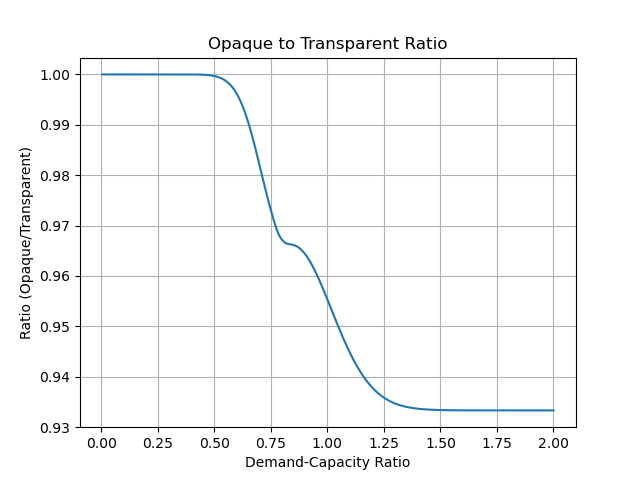
\includegraphics[width=0.5\linewidth]{pic/0930_ratio1.png}
    \caption{$W_i(20,20,20,20,t)$ v.s. $V_i(20,20,t)$}
    \label{fig:ratio1}
\end{figure}


\begin{figure}
    \centering
    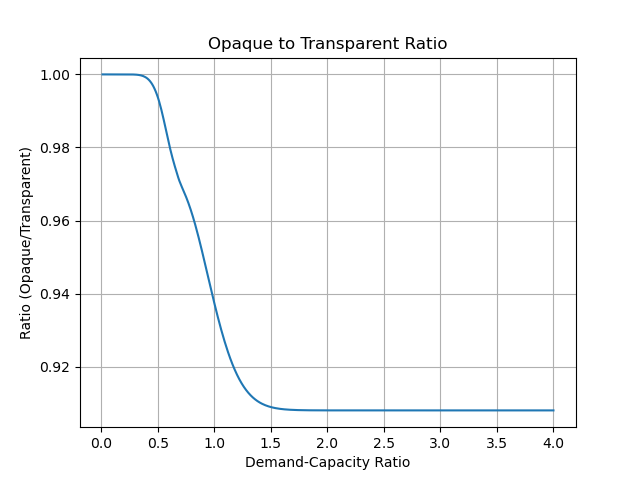
\includegraphics[width=0.5\linewidth]{pic/0930_ratio2.png}
    \caption{$W_i(10,10,10,10,t)$ v.s. $V_i(10,10,t)$}
    \label{fig:ratio2}
\end{figure}

\begin{figure}
    \centering
    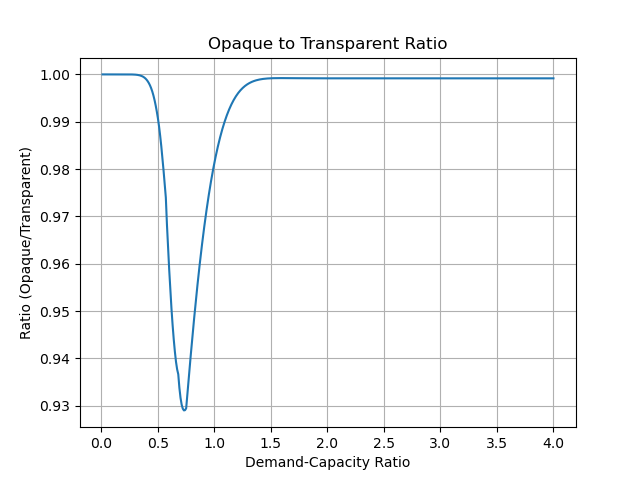
\includegraphics[width=0.5\linewidth]{pic/0930_ratio3.png}
    \caption{$W_i(10,10,20,20,t)$ v.s. $V_i(10,10,t)$}
    \label{fig:ratio3}
\end{figure}

Figure \ref{fig:ratio3} indicates the case when both firms overestimate the initial capacity; we can see that the revenue ratio reapproaches $1$ when the demand-capacity ratio surpasses $1$.

\begin{figure}
    \centering
    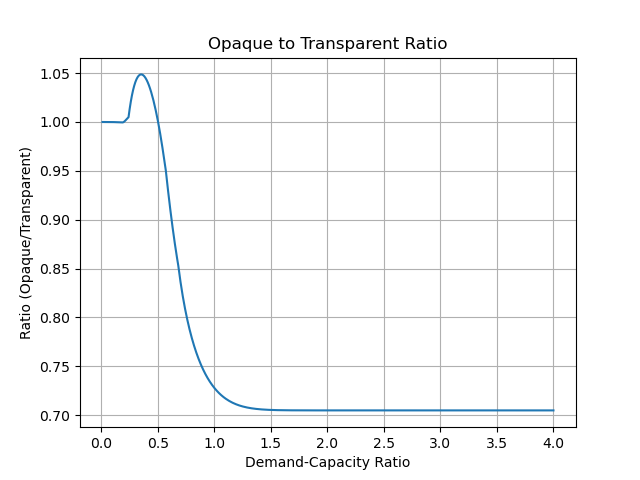
\includegraphics[width=0.5\linewidth]{pic/0930_ratio4.png}
    \caption{$W_i(10,10,5,5,t)$ v.s. $V_i(10,10,t)$}
    \label{fig:ratio4}
\end{figure}

\begin{figure}
    \centering
    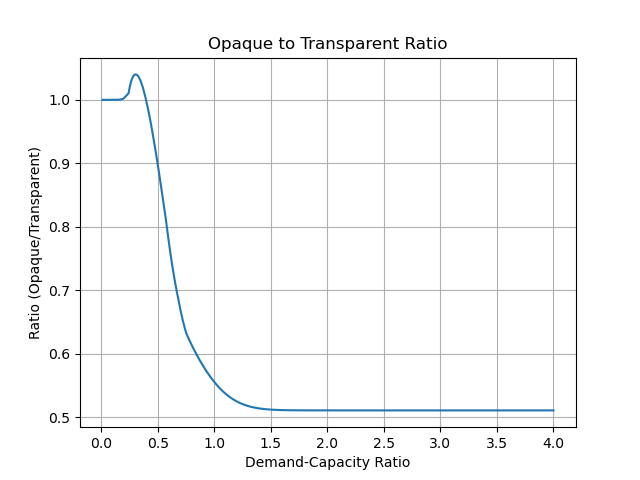
\includegraphics[width=0.5\linewidth]{pic/0930_ratio5.png}
    \caption{$W_i(10,10,5,20,t)$ v.s. $V_i(10,10,t)$}
    \label{fig:ratio5}
\end{figure}

Figure \ref{fig:ratio4} indicates the case when both firms underestimate another firm's initial capacity, and figure \ref{fig:ratio5} indicates the case when one firm underestimates another firm's initial capacity while the other firm overestimates the opponent's capacity.

\subsection{Asymmetric Initial Capacity}

\bibliographystyle{apalike}
\bibliography{reference}
\end{document}